\section{Proposed Method}
\label{sec:proposed_method}
\begin{figure}[b]
    \centering
    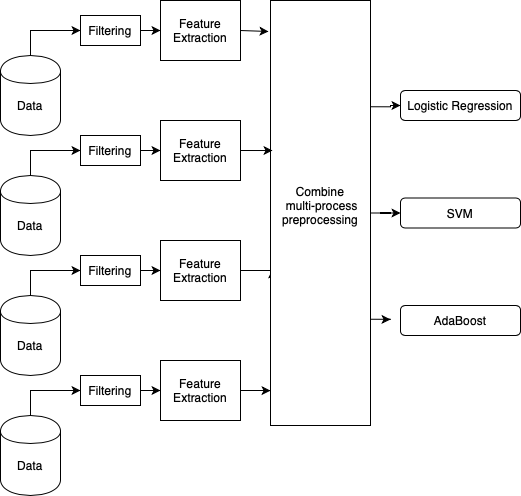
\includegraphics[width=\columnwidth]{tex/figures/model.png}
    \caption{Our Proposed Method}
    \label{fig:model}
\end{figure}

Our preliminary testing found that dataset loading and preprocessing stage was very slow.
To combat this, we designed a multi-processes preprocessing stage.
Here each process reads a chunk of the data and applies filtering,
feature extraction, and dimensional reduction independently.

For filtering, we use a butter worth filter with various cutoffs which are dependent on the signal in which we are processing.
Band notch is used to remove power line hum, and high pass filters are used to remove
baseline wander.
For feature extraction, we split the EEG signal into its alpha, beta, theta, and gamma bands.
From these bands, we then extracted their corresponding PSD and their relative PSD values. Also, across the channels, we compute mean, min, max, and STD to introduce more variance to our features.
For ECG signals, from each hand separately, we extracted IBI, its mean, STD, Skew, and Kurtosis features. Also, PSD and relative PSD were computed for different bands. Moreover, heart rate, its mean, STD, Skew, and Kurtosis was extracted. 
In total, we extracted 384 features from our dataset.
For dimensional reduction, we reduced the 384 dimensions using PCA
and then selecting the top 40 vectors.
Although this is a significant reduction in dimension, we keep 82\% of our
original variance.

Then these processes join and are fed into 4 different classifiers;
A Logistic Regression, linear SVM, AdaBoost and KNN.
We also tried to use Naive Bayes, but the results did not look promising, so we excluded that.
These classifiers are independent, and their output is measured separately. 
It is worth mentioning that we test the KNN model with all Ks in the range of 1 to 25, and
understood that the average number of 9 nearest neighbours works fine for all the emotion categories.
We also feed each model into a voting classifier.
If we had time, we would have continued our multiprocessing efforts to do each
classification in parallel to further reduce run time.